\documentclass[tikz,border=6pt]{standalone}
\usepackage{amsmath}
\usepackage{xcolor}
\usetikzlibrary{arrows.meta,positioning,calc}

\definecolor{axisgray}{HTML}{333333}
\definecolor{lineblue}{HTML}{4A90D9}
\definecolor{linered}{HTML}{E74C3C}
\definecolor{labelgreen}{HTML}{3C763D}

\begin{document}
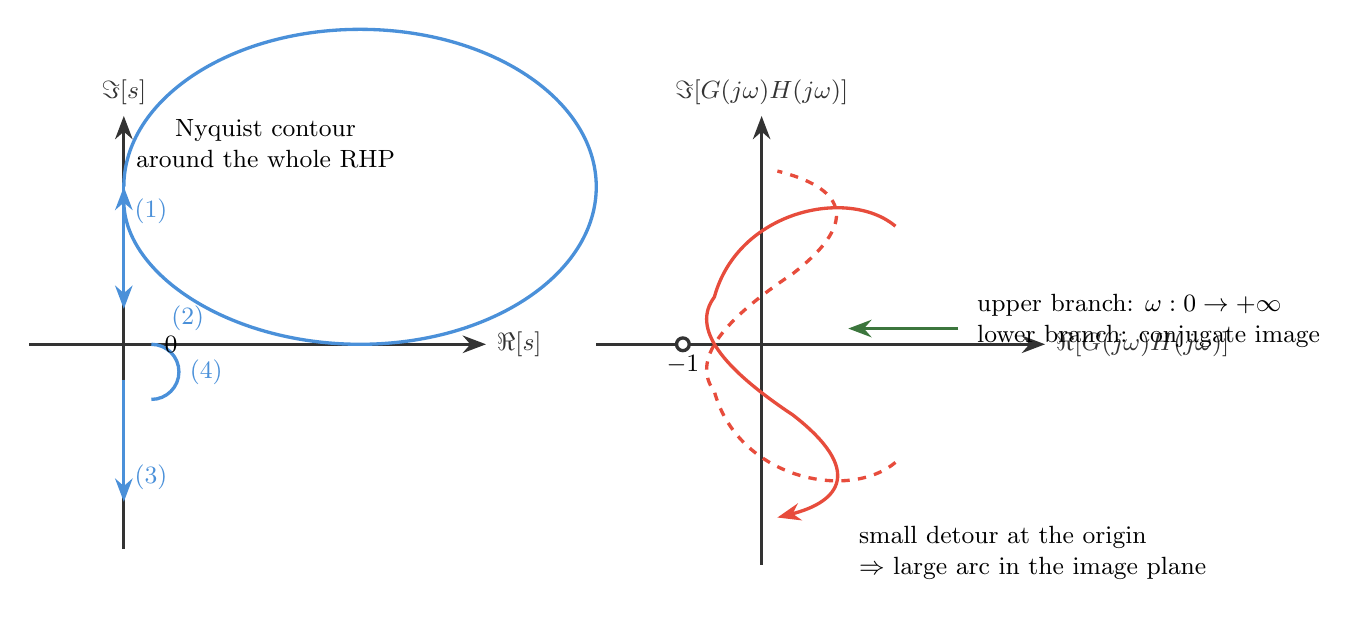
\begin{tikzpicture}[>=Stealth, line width=1.2pt, font=\small]
  \draw[axisgray, ->] (-1.2,0) -- (4.6,0) node[right] {$\Re[s]$};
  \draw[axisgray, ->] (0,-2.6) -- (0,2.9) node[above] {$\Im[s]$};
  \draw[lineblue, ->] (0,2.0) -- (0,0.45) node[pos=0.2, right] {(1)};
  \draw[lineblue] (0.35,0) arc[start angle=90,end angle=-90,radius=0.35] node[midway, right] {(4)};
  \draw[lineblue, ->] (0,-0.45) -- (0,-2.0) node[pos=0.8, right] {(3)};
  \draw[lineblue, ->] (0,2.0) arc[start angle=180,end angle=-180,x radius=3.0,y radius=2.0] node[pos=0.88, below] {(2)};
  \node[align=center] at (1.8,2.55) {Nyquist contour\\around the whole RHP};
  \node[right] at (0.38,0) {$0$};

  \draw[axisgray, ->] (6.0,0) -- (11.7,0) node[right] {$\Re[G(j\omega)H(j\omega)]$};
  \draw[axisgray, ->] (8.1,-2.8) -- (8.1,2.9) node[above] {$\Im[G(j\omega)H(j\omega)]$};
  \filldraw[fill=white, draw=axisgray] (7.1,0) circle (2.3pt);
  \node[below] at (7.1,0) {$-1$};
  \draw[linered, ->] (9.8,1.5) .. controls (9.2,2.0) and (7.8,1.7) .. (7.5,0.6)
    .. controls (7.2,0.2) and (7.6,-0.3) .. (8.5,-0.9)
    .. controls (9.4,-1.6) and (9.1,-2.0) .. (8.3,-2.2);
  \draw[linered, dashed] (9.8,-1.5) .. controls (9.2,-2.0) and (7.8,-1.7) .. (7.5,-0.6)
    .. controls (7.2,-0.2) and (7.6,0.3) .. (8.5,0.9)
    .. controls (9.4,1.6) and (9.1,2.0) .. (8.3,2.2);
  \draw[labelgreen, ->] (10.6,0.2) -- (9.2,0.2);
  \node[align=left, anchor=west] at (10.7,0.3) {upper branch: $\omega:0\to+\infty$\\lower branch: conjugate image};
  \node[align=left, anchor=west] at (9.2,-2.65) {small detour at the origin\\$\Rightarrow$ large arc in the image plane};
\end{tikzpicture}
\end{document}
